\section{Методы формирования трехмерных микро- и наноструктур}

\subsection{Наноимпринтная литография}
Наноимпринтная литография (НИЛ) -- технология, предназначенная для переноса изображения наноструктуры или электронной схемы на полимерный материал путем прямого воздействия на него специальным штампом~\cite{NIL_1, NIL_2}. Существуют два основных метода НИЛ -- термическая и ультрафиолетовая (УФ). В термической НИЛ штамп вдавливается в полимер, нагретый до температур выше температуры стеклования, затем происходит его охлаждение и извлечение штампа. В ультрафиолетовой НИЛ штамп из материала, прозрачного в УФ области спектра, погружается в жидкий полимер, который отверждается под действием УФ излучения, после чего происходит извлечение штампа. Штамп обычно изготавливается из металла или кремния (для термической НИЛ) и полимеров или кварца (для УФ НИЛ) с помощью электронно-лучевой литографии. Учитывая прямой контакт штампа с основным материалом, а также масштаб печати 1:1, к штампу предъявляются повышенные требования по плоскопараллельности и бездефектности.  Перед проведением процесса НИЛ штамп покрывается специальным антиадгезионным покрытием, что позволяет избежать прилипания полимера к штампу при его отделении. Также после печати неизбежно остаётся тонкий остаточный слой полимера, который удаляют с помощью плазменного травления. Преимуществами НИЛ являются простота процесса (при наличии штампа), высокая производительность и возможность достижения высокого разрешения (менее 100 нм). К недостаткам этого метода относятся трудоемкость и дороговизна процесса изготовления штампа надлежащего качества, необходимость частого его обслуживания (удаления остатков основного материала), а также сложность совмещения штампа с низлежащим слоем. Несмотря на то, что технология НИЛ изначально создавалась как альтернатива фото- и электронно-лучевой литографии, она может применяется для получения трехмерных микро- и наноструктур, таких как фотонные кристаллы~\cite{NIL_nanophotonics}, микроканалы~\cite{NIL_microfluidics} и др.~\cite{NIL_3D_1, NIL_3D_2}

\begin{fig}{NIL}{NIL_white_bg}
	Схематическое изображение процессов термической и УФ НИЛ.
\end{fig}

\subsection{Двухфотонная лазерная литография}

Двухфотонная лазерная литография (ДЛЛ) — технология создания микро- и наноструктур, основанная на двухфотонном поглощении внутри фокального объёма лазерного излучения~\cite{Hohmann2015, Kawata2001}. Фотовозбуждение компонент литографической смол приводящее к ее отверждению, происходит лишь в окрестности перетяжки сфокусированного лазерного излучения благодаря нелинейному характеру поглощения. Процесс отверждения имеет пороговый характер, что позволяет регулировать размер отверждаемого объёма, изменяя дозу или плотность энергии поглощённого лазерного излучения. Последующее погружение смолы в растворитель приводит к удалению тех участков, которые не были подвергнуты воздействию излучения. В качестве источника излучения в ДЛЛ обычно используется фемптосекундный лазер, работающий в инфракрасном диапазоне, в качестве литографической смолы -- вещество, содержащее реакционно-способные олигомеры и фотоинициатор. При точной фокусировке ДЛЛ способна обеспечить разрешение менее 1 мкм. Поскольку в ДЛЛ положение центров отвреждения может задаваться произвольно, эта технология нашла применение для формирования трехмерных во многих областях -- микрофлюидике~\cite{TPL_microfluidics_1, TPL_microfluidics_2}, биологии и \break медицины~\cite{TPL_biology_1, TPL_biology_2}, оптике и нанофотонике \cite{TPL_optics, TPL_nanophotonics}, и др. При этом, силу своей природы, данная технология обладает низкой производительностью, что является ее главным недостатком.

\begin{figure}
	\centering
	\begin{subfigure}{.5\textwidth}
		\centering
		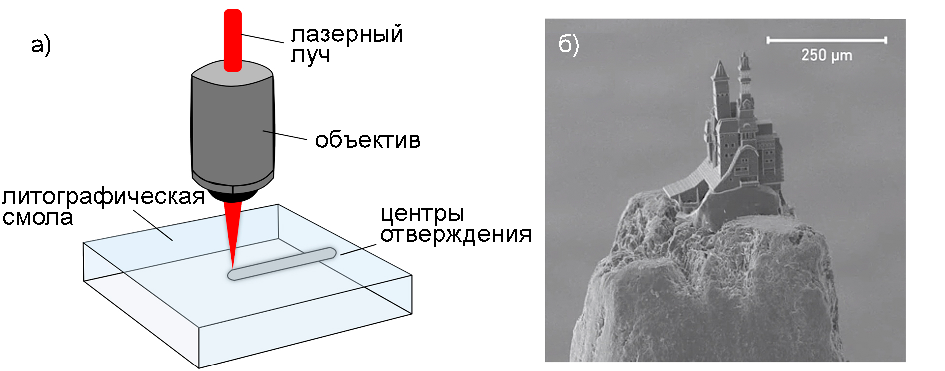
\includegraphics[width=.95\linewidth]{TPL}
	\end{subfigure}%
	\begin{subfigure}{.5\textwidth}
		\centering
		\includegraphics[width=.95\linewidth]{TPL_structure}
	\end{subfigure}
	\caption{Схематическое изображение процесса ДЛЛ и пример структуры.}
\end{figure}


\subsection{Интерференционная литография}

Интерференционная литография (ИЛ) -- метод формирования периодической структуры в резисте, основанный на экспонировании резиста пространственно упорядоченным стоячим электромагнитным полем, возникающим при интерференции двух и более когерентных монохроматических или квазимонохроматических пучков излучения~\cite{IL_general}. Когерентность интерферирующих пучков обычно обеспечивается путем разделения исходного когерентного пучка на соответствующее число пучков с помощью различных интерференционных схем. При наноструктурировании ИЛ применяется для получения  метаматериалов~\cite{IL_metamaterials}, нанофотонных и наноплазмонных устройств~\cite{IL_nanophotonics}, биомедицинских объектов~\cite{IL_biomedical}, изделий на основе выращиваемых наноэлементов и самоорганизующихся структур~\cite{IL_self-assembly} и др.
В оптическом и УФ-диапазонах используются зеркальные схемы (Френеля, Ллойда и др.), схемы на преломляющей оптике (бипризма Френеля, билинза Бийе) или комбинированные зеркально-линзовые схемы. В этих диапазонах в качестве источника исходного пучка с высокой степенью монохроматичности и когерентности используются мощные лазеры, позволяющие получить разрешение до 100 нм. Вопрос обеспечения высокого разрешения ИЛ решается путем перехода в область рентгеновского излучения~\cite{IL_X-ray}. К недостаткам метода можно отнести не самую высокую производительность и возможность получения исключительно периодических структур.

\begin{figure}
	\centering
	\begin{subfigure}{.5\textwidth}
		\centering
		\includegraphics[width=.95\linewidth]{IL_1}
	\end{subfigure}%
	\begin{subfigure}{.5\textwidth}
		\centering
		\includegraphics[width=.95\linewidth]{IL_2}
	\end{subfigure}
	\caption{Схематическое изображение процесса ИЛ.}
\end{figure}


\subsection{Полутоновая литография}

Полутоновая литография (ПЛ) -- общее название для методов, позволяющих получить сложный трехмерный рельеф в резисте в литографическом процессе с одной одной стадией экспонирования~\cite{GL_general}. В их основе лежит пространственная модуляция дозы при экспонировании, приводящая к локальному увеличению или уменьшению скорости растворения резиста при проявлении. Таким образом, конечный рельеф имеет ступенчатую форму и состоит из участков резиста, растворенных в различной степени. Сглаживание границы между участками, проэкспонированных с различными дозами, может быть в дальнейшем достигнуто за счет оплавления образца при температурах вблизи его температуры стеклования. При этом существующие методы моделирования эволюции поверхности полимеров при их оплавлении позволяют использовать этот процесс как дополнительный этап структурирования~\cite{Kirchner_reflow}. Таким образом, полутоновая литография с последующим оплавлением образца является гибкой технологией микро- и наноструктурирования, использующейся в оптике и нанофотонике~\cite{GL_optics}, микрофлюидике~\cite{GL_microfluidics}, формировании микроэлектромеханических систем~\cite{GL_MEMS} и других областях. Существует как электронно-лучевая, так и фото-ПЛ, однако, фото-ПЛ имеет некоторые ограничения, связанные с оплавлением резиста. Так, например, вязкость широко распространенного негативного фоторезиста SU-8 при экспонировании увеличивается, что усложняет процесс контролируемого оплавления~\cite{Kirchner_GL_review}. К недостаткам метода можно отнести его сложность и производительность, еще более низкую, чем при электронно-лучевой и фотолитографии за счет дополнительной стадии оплавления образца.

\begin{figure}
	\centering
	\includegraphics[width=.95\linewidth]{GL_process}
	\includegraphics[width=.45\linewidth]{GL_examples}
	\caption{Схематическое изображение процесса ПЛ и примеры структур.}
\end{figure}


\subsection{Сканирующая зондовая литография}

Сканирующая зондовая литография (СЗЛ) включает в себя семейство технологий формирования структур с наноразмерным разрешением. Каждая из технологий основана на применении специального сканирующего зонда для воздействия на поверхность образца, приводящего к локальным изменениям поверхности. В зависимости от природы воздействия зонда на поверхность можно выделить следующие основные виды СЗЛ:
\begin{itemize}
	\item механическая, в которой изменение поверхности образца происходит в результате механического воздействия зонда ~\cite{SPL_mechanical};
	\item  термохимическая, в которой воздействие нагретого зонда на образец приводит к термической активации различных химических реакций в нем~\cite{SPL_termochemical};
	\item СЗЛ с приложением напряжения, при которой высокая напряженность электростатического поля в области зонда приводит к разложению молекул жидкости~\cite{SPL_bias_liquid} или газа~\cite{SPL_bias_gas}, окружающего образец, и локальному отложению материала на образце;
	\item окислительная СЗЛ, основанная на модификации поверхности путем ее локального окисления~\cite{SPL_oxidation};
	\item перьевая СЗЛ, в которой сканирующий зонд используется для нанесения на поверхность образца органических, полимерных или коллоидных наночернил~\cite{SPL_dip_pen_1, SPL_dip_pen_2}
\end{itemize}

Поскольку сканирующий зонд воздействует только на поверхность образца, этот метод может быть использован только для послойного формирования рельефа (в отличие от, например, ДЛЛ). Однако, высокое разрешение этой технологии и возможность ее реализации с использованием различных материалов обеспечили ей широкое применение. При этом, как и ДЛЛ, производительность сканирующей зондовой литографии крайне низка.

\begin{narrowfig}{SPL}{SPL}
	Диаграмма, отображающая различные реализации метода СЗЛ.
\end{narrowfig}


\section{Блок-сополимеры}


\section{Методы на основе цепной деполимеризации резиста}
Процесс цепной деполимеризации полимерных молекул~\cite{depol_general_1}, обратный процессу полимеризации, может быть использован для формирования рельефа в полимерном резисте. Цепная реакция деполимеризации резиста становится возможна при повышенных температуре (выше температуры стеклования резиста), и для инициирования этого процесса требуется нарушение целостности главной цепи полимерной молекулы, приводящее к радикализации концов молекулы в месте разрыва~\cite{depol_general_2}. В процессе цепной деполимеризации резиста от полимерной молекулы последовательно отделяется большое число мономеров (по разным данным от нескольких сотен до нескольких тысяч~\cite{Madorsky, Mita_PMMA_zip_lengths_T, Inaba_zip_len}), который вследствие диффузии покидает область, в которой находилась молекула. Это приводит к образованию свободного пространства в резисте, что и позволяет использовать этот процесс для микро- и наноструктурирования.

Существуют два устоявшихся подхода в области формирования трехмерного рельефа в резисте на основе процесса цепной деполимеризации. В каждом из них нагревание резиста происходит локально, что ограничивает область деполимеризации резиста. Первый подход по своей сути является термической сканирующей зондовой литографией, в который для разрушения целостности полимерных молекул используется нагретый зонд~\cite{depol_fabrication_probe}. Разрывы молекул в этом случае происходят случайно за счет повышенной температуры резиста. Во втором подходе используется сфокусированный лазерный луч, который вызывает локальный нагрев резиста и разрушение в главной цепи его молекул~\cite{depol_fabrication_laser}.

Однако, существует еще один подход, основанный на нагреве всего образца, что позволяет реакции цепной деполимеризации протекать в любой его области, при условии возникновения активного центра деполимеризации. На нем основан метод термостимулированной электронно-лучевой литографии, в котором резист при температуре выше его температуры стеклования экспонируется электронным лучом. Отличительными особенностями этого метода является высокая производительность и возможность формирования двух- и трехмерных профилей в резисте с высоким разрешением по вертикали. Описанию состояния этого метода на текущий момент будет посвящена вторая часть этой главы.








